

\documentclass{article}
\usepackage[utf8]{inputenc}
\usepackage{authblk}
\usepackage{adjustbox}
\usepackage{enumerate}
\usepackage{setspace}
\usepackage[margin=1.25in]{geometry}
\usepackage{hyperref}
\usepackage{csvsimple}
\usepackage{graphicx}
\graphicspath{ {./figures/} }
\usepackage{subcaption}
\usepackage{amsmath}

%%%%%% Bibliography %%%%%%
% Replace "sample" in the \addbibresource line below with the name of your .bib file.
\usepackage[style=nejm, 
citestyle=numeric-comp,
sorting=none]{biblatex}
\addbibresource{refwork.bib}

%%%%%% Title %%%%%%
\title{ECS 189G: Numerical Approximation for Categorical Data in Evaluating Risk of Drug Consumption}

%%%%%% Authors %%%%%%
% Authors should be listed in order of contribution to the paper, by first name, then middle initial (if any), followed by last name.
% Authors should be listed in the order in which they will appear in the published version if the manuscript is accepted. 
% Use an asterisk (*) to identify the corresponding author, and be sure to include that person’s e-mail address. Use symbols (in this order: †, ‡, §, ||, ¶, #, ††, ‡‡, etc.) for author notes, such as present addresses and similar information.
% You can include group authors, but please include a list of the actual authors (the group members) in the Supplementary Materials.
\author[$\S\dag$]{Arjun Ashok}
\author[$\S$]{Benjamin Stone}
\author[$\S$]{Thalia Fay}
\author[$\S$]{Mohammad Ahmed}

%%%%%% Affiliations %%%%%%
\affil[$\S$]{College of Letters \& Sciences, University of California, Davis, Davis, CA}
\affil[$\dag$]{Corresponding Author, arjun3.ashok@gmail.com}

%%%%%% Date %%%%%%
\date{June 13th, 2023}

%%%%%% Spacing %%%%%%
% Use paragraph spacing of 1.5 or 2 (for double spacing, use command \doublespacing)
\onehalfspacing

\begin{document}

\maketitle

%%%%%% Abstract %%%%%%
\begin{abstract}
The rising prevalence of drug use and its corresponding implications on key societal aspects, notably employment, demands the formulation of improved methodologies for accurately predicting drug consumption. To address this need, we undertake an exploratory journey into a dataset comprising numerical personality test results paired with categorical drug usage survey data. Our goal goes beyond mere prediction; we seek to construct a machine learning model that efficiently anticipates an individual's most recent drug usage occurrence while ensuring equitable treatment of sensitive variables such as gender, age, and race. This distinctive pursuit of balance minimizes potential biases that could inadvertently manifest in the model. Our methodology includes selectively removing and judiciously scaling down certain features, and meticulously transforming categorical data into a numerically compatible format.


Our investigation not only aligns with but also bolsters the findings of our reference study. We independently identified similar personality traits that serve as significant predictors for each specific drug. Intriguingly, like the comparative study, we discovered that gender proves to be an invaluable predictive feature. However, our path diverges from theirs at the point of ensuring fairness in our model. In an innovative departure, we deliberately scaled down the weight of the gender feature to enhance the fairness of our model. This critical adjustment assumes a heightened level of importance, particularly in scenarios like employment where such a model could conceivably be deployed. In the effort to create a more balanced predictive model that does not compromise on accuracy, we tackled the challenge of handling categorical predictive variables by converting them into numerical counterparts. This alternative one-hot encoding method enabled us to harness the detailed information enclosed in categorical data while maintaining compatibility with numerical computation methods. This innovative process allowed us to incorporate previously incompatible data into our predictive model, enhancing the unique blend of accuracy and fairness that characterizes our study. As such, our work not only offers a promising foundation for future research in this field but also presents a feasible model for real-world applications, underscoring the realistic possibility of achieving balance in predictive modeling.

\end{abstract}


%%%%%% Main Text %%%%%%
%%%%%% Introduction %%%%%%
\section{Introduction}
    \subsection*{Background and Terms}
    Unlike the accompanying paper by E. Fehrman et al. which we will frequently reference, we will not first define the basis for classifying a chemical as a drug. What we aim to provide with this paper is not analysis of personality tests and their bearing on drug consumption, but rather an improved methodology for predicting the consumption of drugs based on a set of features. In this regard, our paper serves more to construct an application of machine learning in balancing the fairness and utility modeling the relationship between personality, gender, age, race, etc. and drug consumption with respect to different drugs, rather than simply studying the predictive power these models can generate.

    With this in mind, we can begin to define some of the key machine learning terms we employ through the paper. First, consider the \textit{fairness-utility} trade-off that states an inherent trade-off exists between balancing the fairness of a model versus the utility it gives with respect to predictive ability. The implication of course being, we have to decide which one of the two to favor in the construction of our model. With regards to drug consumption, it benefits potential users of the model (e.g. employers, police) to maintain fairness with respect to several \textit{sensitive} features such that there exists as little bias as is reasonable.

    By \textit{sensitive} features, we are addressing the information in the dataset that may serve to create inherent biases towards marginalized groups. In other words, sensitive features contain data that may be useful for improving the predictive power of our model, but comes at a price of fairness. Any time we use a sensitive feature, we have to be wary of the bias it induces in our model.

    \textit{One-Hot encoding} is a technique used frequently with categorical data in machine learning to enable model training. The process consists of splitting apart the unique values of a categorical variable (i.e for 'animals' we might split them into 'dog', 'cat', etc.) and then recording whether (yes is a 1) or not (no is a 0) the split category is identified. In more technical terms, we split a single feature into a vector of 0's and 1's for each 'dummy' feature, where every vector will have a single 1 and others are 0, allowing us to predict for every case. The motivation behind encoding is the loss of information that comes from just representing each category as a number. If 'dog' was a 1, 'cat' was a 2, 'horse' was 3, etc. then a model we train to would misinterpret the category as being numerical and create misguided predictions based on this assumption.

    One thing of note to mention, however, is the one-hot encoding creates a number of new features, potentially increasing the risk of over-fitting with datasets (such as ours) which already contain a significant amount of features in proportion to the number of entries.


    \subsection*{Relevance and Importance}
    Over the last decade, it has become common practice for large companies to use artificial intelligence to cull undesirable individuals from large applicant pools. While this seems logical, using machine learning models to predict undesirability introduces numerous opportunities for unseen hiring discrimination against people who, for no fault of their own, trigger poor results from a model. Without oversight of these new hiring practices, there is inherent risk that people will be discriminated against on the basis of gender, age, or race.

    While neither our model nor the model of the researchers have likely yet been deployed by employers to predict the likelihood of an applicant being a drug user, it is really not far fetched considering more than 75 percent of large companies already use personality tests during the hiring process \cite{Claypool}. These companies will typically evaluate the results manually to select for people they think will be good matches. Importantly, though, this process could easily be automated through a machine learning model that has been trained to notice good candidates by using their personality test results to predict metrics applicable to the work environment like drug usage. We have no doubt that if such an algorithm existed with high accuracy, then employers would use it to flag risky applicants.

    In this realistic scenario, it is critical that issues of fairness do not become completely abstracted behind an algorithm. For example, if gender was used in a black-box model predicting drug usage, then there may exist a hidden slant against men or women based on which gender uses drugs like cannabis or alcohol more often. Additionally, while it is unlikely a licensed model would explicitly use race as a predictor, features such as education level and birthplace may inevitably serve as proxies for race, causing certain groups to be disproportionately predicted for usage. We have thus sought to carefully explore how such a potentially useful product for employers could be modified to ensure fairness.

    
    \subsection*{Proposed Solution}
    Our proposed solution to combat the shortcomings of Fehrman's study in weighting fairness above utility is a combination of a few key strategies:
    \begin{enumerate}[I]
        \item Deweighting sensitive variables and their proxies to balance the utility we get from the information they provide with the bias induced within the model. This is done through an iterative process to get the optimal deweighting factors.
        \item Constructing numerical representations of the drug consumption to minimize features and allow for more interpolation between predictions, enabling more nuanced predictions.
        \item Scaling and reframing the output of the model in such a way that risk is better reflected, allowing for easier interpretations from analysts.
    \end{enumerate}
    

    \subsection*{Outline}
    Over the course of this paper, we'll first explore the dataset in-depth to fulyl recognize the behavior and information the data we are working with possesses. Next, we'll consider the differing methodologies in our implementation with K-Nearest Neighborss regression modeling versus the categorical modeling with one-hot encoding used by Fehrman \cite{Fehrman}. Finally, we'll independently evaluate the models' performance against the metrics Fehrman produce, as well as some of our own to ensure we meet the outlined goals regarding the balance of fairness and utility. In this evaluation, we'll outline how our approach may eventually be applied to other mediums and datasets for better a better fairness-utility balance.
    

% %%%%%% Figures %%%%%%
% \subsection*{Figures}
% Figures should be called out within the text and numbered in the order of their citation in the text. Every figure must have a descriptive title beginning with ``Figure [Number] …'' All figure titles should be either a phrase or a sentence; do not mix the two styles. See Figure \ref{fig:1} for example.
% \begin{figure}[h]
%     \centering
%     \includegraphics[width=0.5\textwidth]{fig 1}
%     \caption{This is an example figure.}
%     \label{fig:1}
% \end{figure}

% \begin{figure}[h]
%     \centering
%     \begin{subfigure}{0.4\textwidth}
%         \includegraphics[width=0.9\textwidth, height=2in]{fig 1}
%         \caption{\label{fig:2a}}
%     \end{subfigure}
%     \begin{subfigure}{0.4\textwidth}
%         \includegraphics[width=0.9\textwidth, height=2in]{fig 2}
%         \caption{\label{fig:2b}}
%     \end{subfigure}
%     \caption{This is an example of a figure consisting of multiple panels.     (\subref{fig:2a}) This is the first panel. (\subref{fig:2b}) This is the second panel.}
%     \label{fig:2}
% \end{figure}


%%%%%% Tables %%%%%%
% \begin{table}[b]
%     \caption{This is an example table.}    
%     \centering
%     \begin{tabular}{ccc}
%             \hline
%             Column 1 & Column 2 & Column 3 \\  
%             \hline
%             Cell 1 & Cell 2 & Cell 3\\ 
%             Cell 4 & Cell 5 & Cell 6 \\
%             \hline
%             \end{tabular}

%     \label{tab:1}
% \end{table}


%%%%%% Dataset Exploration %%%%%%
\section{Dataset Exploration}
The dataset we use is sourced from Scutari's FairML package for R and the paper by E. Fehrman et al. The dataset consists of 1885 entries and 31 features, including the predicted features. A large proportion of the dataset is made up from those with higher drug consumption habits as a byproduct of the data being collected specifically for this study. The paper acknowledges that the sample collected from the survey is biased towards a higher proportion of drug users, meaning the percentage of drug users in the general population is significantly lower. The use of this sample is justified by mentioning how such a bias is common in clinical cohorts, thus the original authors proceeded with risk evaluation \cite{Fehrman}.

The dataset was missing no information, meaning it was not necessary to impute data for any of the features. Additionally, the choice was made to avoid oversampling the minorities not represented by some of the more sensitive features (Race in particular) since the diversity was so limited we would be better off disregarding the feature completely. Furthermore, not oversampling was done for the predictive variables for drug consumption as the dataset contains a large majority of drug users, but a significant minority of low-medium drug consumers as well.

The sensitive features found include Age, Gender, and Race. Close proxies to the previously listed appear in the form of Country and Education for Race, and certain personality traits such as Impulsivity and Sensation-Seeking for Gender and Age. Age, Gender, Race, Country, Education, and all drug consumptions are the categorical features in the dataset, while Nscore, Escore, Oscore, Ascore, Cscore, Impulsive, and SS are the numeric features.

In terms of feature distribution, it seems the Age distribution is skewed more towards age groups from 18 - 55, meaning any bias that we encounter may simply be an artifact from this bias in the data. Gender, on the other hand, was almost evenly split, so any bias encountered would likely indicate a biased model. Education was skewed heavily towards those who either attempted or finished higher education beyond high-school, possibly indicating a relationship between the age distribution (each generation typically has seen an increase in education rates) and therefore a proxy for age. Country and Race seem to be heavily concentrated on US and UK inhabitants who are white, meaning any bias induced with race is unlikely given the complete lack of data with race.

With these distributions in mind, we can effectively neglect to consider race and country as factors as at all since their categorical nature will increase the number of features considered, potentially creating an overfitted model, and the information they provide to us and the model will not offset the potential bias in any way. Fehrman employs a similar approach with regards to neglecting race and countries for these reasons \cite{Fehrman}. Fehrman also neglects to use age at all similar to our approach of using education to approximate age given there high correlations \cite{Fehrman}.    

In terms of predictions, the drug consumption variables are stored as a factor variable, from "never used [drug] before" to "used within the last day". Each drug usage is predicted on by a separate model, allowing these to function simultaneously as features for other drug consumption prediction as well as the predictive variable for its own drug consumption.

%% Correlation Matrices %%
\begin{figure}[ht]
    \centering
    \begin{subfigure}{0.4\textwidth}
        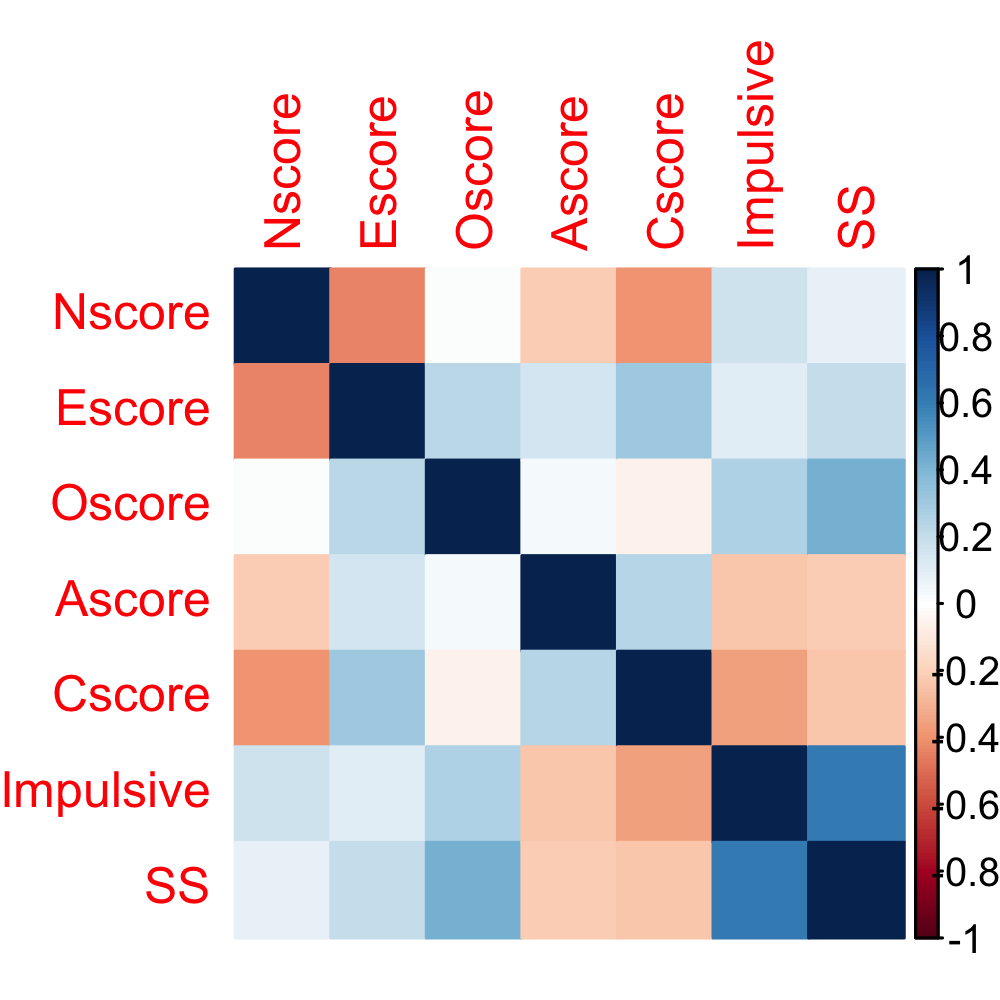
\includegraphics[width=0.9\textwidth, height=2in]{figures/num_correlation_plot.png}
        \caption{\label{fig:num_corr}}
    \end{subfigure}
    \begin{subfigure}{0.4\textwidth}
        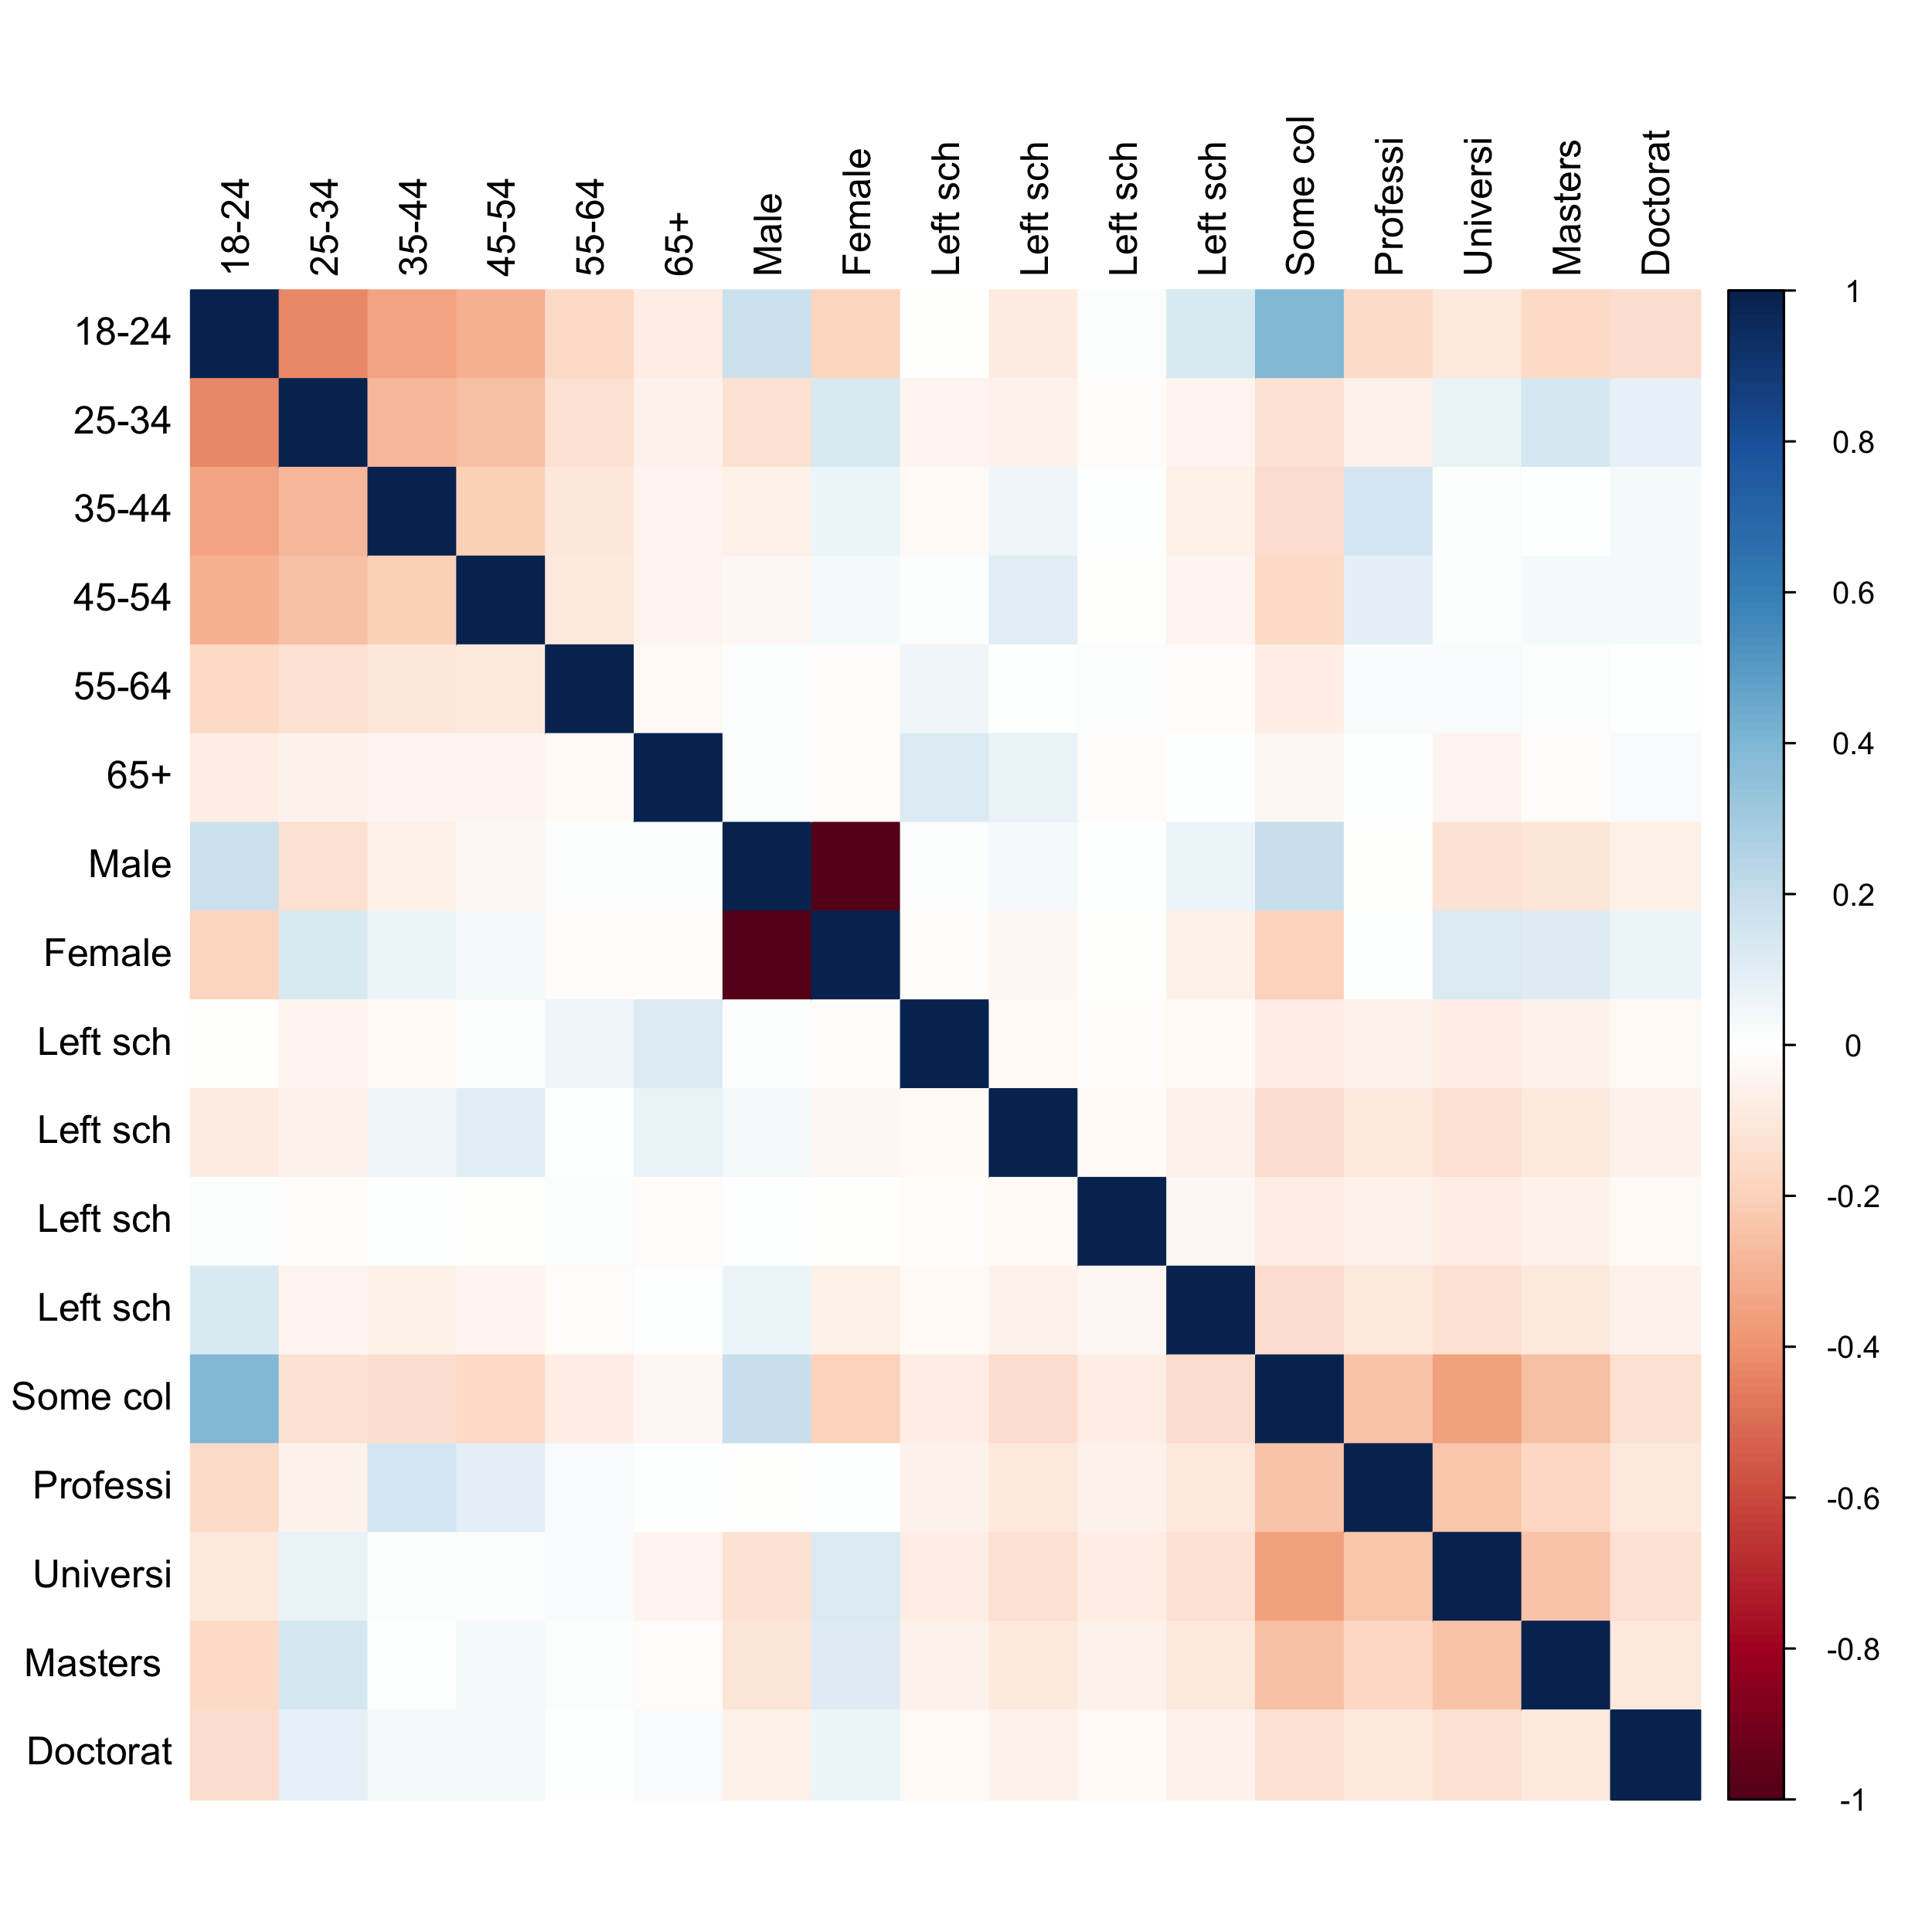
\includegraphics[width=0.9\textwidth, height=2in]{figures/cat_correlation_plot.png}
        \caption{\label{fig:cat_corr}}
    \end{subfigure}
    \caption{The correlations between the numerical (using Pearson correlation) and categorical (one-hot encoding w/ Kendall correlation) features are shown here separately}
    \label{fig:1}
\end{figure}


%%%%%% Methodology %%%%%%
\section{Methodology}
    \subsection{Prior Work}
    Fehrman et al. employed different methods to evaluate the risk of drug consumption. These methods were: k-Nearest Neighbors, Decision Tree, Linear Discriminant Analysis, Gaussian Mixture, Probability Density Function Estimation, Logistic Regression, Naive Bayes and Random Forest \cite{Fehrman}.

    The original authors chose the best classifier through the usage of Leave-One-Out cross validation (LOOCV) \cite{Fehrman}. LOOCV was done to determine which classifier yielded the smallest difference between sensitivity and specificity. Further computation was done in the event that two classifiers had the same minimum between sensitivity and specificity, where they selected the classifier with the higher sum of sensitivity and specificity. It is worth nothing that classifiers with sensitivity and specificity of less than 50\% were not considered. Nearly all the sensitivity and specificity values were above 70\% for all classification tasks, with the best results (over 75\%) achieved for cannabis, crack, ecstasy, legal highs, LSD, and volatile substance abuse (VSA).

    % edit to fit flow
    Key to our analysis, the researchers did not remove features like race and gender from their models for the purpose of fairness. Rather, features were selected purely for utility. Despite this choice, race and country of origin ended up being removed from every single model, primarily because there was not enough data from non-whites and people from outside of the US and UK to make such features good predictors. On the other hand, gender, age, or education were used as a predictor for the majority of the final models.

    
    \subsection{Data Engineering}
    In contrast, our solution takes a very data-engineering-heavy approach. First, we take special care in constructing numerical representations of our drug consumptions data. The intuition behind this step comes from the underlying numerical basis for each level in the categorical feature. Since the usage data corresponds to different time-frames, we can replace each time frame not with basic integers such as in integer encoding, but rather specific ratios that relate directly to the levels they describe. Additionally, these ratios should correlate in some sense to risk: the higher the ratio, the more risk is predicted, and vice-versa.
    
    Following the above blueprint, we have theorized the Numerical Approximation for Categorical Data (NACD). In NACD, we essentially conduct the following steps. Take a specific time-frame to be the base. This time-frame will equate to $1$ in the final ratio. To calculate any time-frame above it (longer time-frame), we simply divide by the corresponding ratio. In our tests, we found that using the 1 year ("used within the last year") to be a useful base. So, relative to this base, the "used in the last decade" level would become $1 * \frac{1}{10}$ to convert from years to decades. This has the added bonus of mapping to risk exactly how laid out previously: as the last usage date grows higher, the outputted consumption number drops sharply. Now consider the opposite, what happens when we perform the same steps for the shorter time-frame? We simply \textit{multiply} by the ratio for each time frame. So, for example, "used in the last month" would become $1 * \frac{12}{1}$ for the 12 months in every year. Once again, there is a sharp increase in this drug consumption number, mirroring the behavior we would expect from risk.

    The ultimate result of this alternative to the one-hot encoding as used by the original authors is a system that manages to capture the non-linear growth in the risk we predict of drug consumption, all the while allowing for numerical interpolation since we can now employ K-Nearest Neighbors regression models to fit the data.

    The next steps we take are a little less elegant. We then drop two columns we had previously deemed useless given their distributions and susceptibility to inducing bias, "Race" and "Country".
    
    Finally, we convert the categorical features that are \textit{not} being predicted into their one-hot encoded forms, dropping the original columns in the process. This allows us to use this categorical information in a meaningful way in our regressive model. Why not use the numerical representation method we had described before? The benefits would not be as great since as large portion of its utility comes from deploying a regressive model over a classifier. Additionally, the remaining features didn't have as strong an underlying numerical basis as did the drug consumption data, meaning the results would not have been as useful.


    \subsection{Numerical Approach for Modeling}
    For our model, we chose to deploy a KNN regression model using the qeML package in R (developed by Professor Matloff). Throughout the modeling process, we experimented with different hyperparameters, namely the deweighting parameter for each of the sensitive features (Gender, Age) and proxies (Education).

    Ultimately, the results of this modeling were enabled to be more precise in their predictions through the use of regression over classification. We are now enabled to see exactly how much risk is being posed by each of the candidates thanks to the weighted numerical approximation technique we described above.


%%%%%% Evaluation %%%%%%
\section{Evaluation}
    \subsection{Evaluation Criteria}
    Measuring fairness is a very nuanced task that requires complex analysis to correctly perform. Furthermore, Fehrman et al. had made the decision to not benchmark fairness in their work, likely citing their disregarding of Age and Race (but not gender) as reason for doing so. With this context in mind, we decided to proceed with simplistic measures of fairness that would ultimately show relationships with biased variables in a digestable metric, rather than more complex metrics. The metric we consider for fairness as such is the Kendall correlation between the sensitive variable and our predicted output. Since Race is irrelevant to the discussion because of the negligible variation in the large majority of entries, we need not consider it at all as a sensitive variable even though its proxy exists in the form of Education.
    
    For the performance evaluation, we are using a combination of our own metrics and the metrics Fehrman et al. use in their analysis, thus providing a better comparison and more in-depth look at our own modeling. Our own metric consists of the qeML default Mean Absolute Prediction Error (MAPE) since we predict on a regressive model. The metrics Fehrman uses consists of sensitivity (true positive rate) and specificity (true negative rate) to measure how often the test predicts the opposite of what was intended. Since those metrics are geared towards classification models, we rate a prediction as positive (1) for the weight it lies directly above (i.e. output of .001 would be classified as "used over a decade ago" or "never used", depending on if .001 was greater than the cutoff or not).

    \subsection{Prior Work}
    \subsubsection{Personality Test}
    Pearson's Correlation was used to determine the association between two personality factors. Results show that all pairs except two demonstrated significant correlation. The unrelated pairs were N and O (\emph{r}=0.017, \emph{p}=0.471) and A and O (\emph{r}=0.033, \emph{p}=0.155).
    
    \subsubsection{NEO Five-Factor Inventory (NEO-FFI-R) scores and Drug Consumption}
    \begin{equation}
        \text{T-score} = 10 \Bigl[\frac{\text{Raw score} - \text{Normative mean score}}{\text{Normative standard deviation}}\Bigr] + 50
    \end{equation}
    The following subdivision was used for the T-score: 44-49 indicates a moderately low score (-), 49-51 indicates a neutral score (0), and 51-56 indicates a moderately high score (+). The N and O scores of users of all 18 drugs were either high (+) or neutral (0), while the A and C scores for all drug users were either low (-) or neutral (0). 
    
    E scores had a specific effect depending on the drug. The E score of users is moderately low (-) for amphetamines, amyl nitrite, benzodiazepines, heroin, ketamine, legal highs, methadone, and crack, moderately high (+) for cocaine, ecstasy, LSD, magic mushrooms, and VSA, and neutral (0) for all the legal drugs.

    \subsection{Performance in Fairness and Utility} 
    %% Tables %%
    \begin{table}
        \centering
        \csvautotabular{figures/model_evaluation.csv}
        \caption{Results from NACD Modeling w/ KNN}
        \label{tab:evaluation_table}
    \end{table}

    %% Analysis %%
    Shown above in Figure \ref{tab:evaluation_table} are the results of our NACD modeling in action. In terms of fairness, lower score being lower correlation being better, we focused on Gender primarily as our comparison, though we took a weighted average of all metrics. This has resulted in quite good mitigation of bias, with most models producing insignificant amounts of skew in the final correlations. In terms of sensitivity, we yielded quite poor scores overall, perhaps due to artifacting from the NACD conversion from categorical to numerical data and back. In terms of specificity, our model performed extremely well, though this may be an indication of improper training due to many perfect results.


    \subsection{Conclusion}
    Overall, the results are somewhat disappointing in regards to the efficacy of our novel approach in tackling drug consumption prediction, However, given our initial goal to create a more balanced model, this approach shows promise in keeping fairness at a high enough balance to warrant the lower accuracies.

    With regards to differing analyses, Fehrman et al. and ourselves conclude similar techniques are necessary in order to properly examine and predict on the drug consumption dataset. While we took a new road with exploring the NACD technique, it serves to show that more established techniques such as one-hot encoding show more promise for now. Given time, however, NACD could develop into a rivaling method for engineering data to give more informative predictions.


%%%%%% Acknowledgements %%%%%%
\section{Acknowledgements}
    \subsection*{General}
    We would like to extend a thank you to Professor Matloff at the University of California, Davis for his work in teaching our background in fair machine learning and preparing us to write our own research paper.
    
    \subsection*{Author Contributions} 
    A. Ashok wrote the entirety of the supporting code for data exploration, analysis, and modeling, as well as conceived of the novel approach NACD. For the paper, he wrote the majority of analysis and methodology in the paper and was in charge of outlining, editing, and leading the research paper. \\
    B. Stone came up with the idea of applying the drug data set to the real life scenario of employers using personality tests to evaluate applicants. He wrote all of the paragraphs that reference and explain this scenario, and he contributed to the sections explaining and analyzing the comparison paper.\\
    T. Fay determined the methodology and evaluation methods used in the accompanying paper, and wrote the reports under the corresponding sections. \\
    M. Ahmed wrote the entirety of the abstract section for the paper and gathered in-depth details from the origin paper where the data set was housed. He also spoke with two student-interns at InRecovery, a company whose goal is to help with drug abuse/rehabilitation. \\


%%%%%% Our Materials %%%%%%
\section*{Supplementary Materials}
You can find all materials in \href{https://github.com/ArjunAshok17/ECS-189G/tree/7dc23ae5986f590f51ca1c3195e4d9f95c2f2f11/TermProject}{A. Ashok's Github Repository}, including but not limited to:
\begin{itemize}
    \item Supporting code for the data exploration in `explore.R`
    \item Supporting code for any utility functions used in `utility.R`
    \item Supporting code for the evaluation criteria used in `metrics.R`
    \item Supporting code for the novel modeling technique in `fair\_analysis.R`
    \item Planning documents for analysis and paper write-up in `analysis\_plan.md`
    \item PDF(s) of the prior work in this area we have addressed
    \item Dataset analyzed
    \item Tex file for the paper
    \item PDF of our paper
\end{itemize}

\printbibliography

\end{document}
